\documentclass[11pt]{article}

\usepackage{fullpage}
\usepackage{graphicx}
\usepackage{amsfonts}
\usepackage{hyperref}


\begin{document}
\title{Hyperion Memo: Assembling a Signal Chain for High Frequency Experiment}
\author{Raj Biswas\\rbiswas@berkeley.edu \and Nipanjana Patra \\nipanjana@berkeley.edu }

\date{December 1,2017}
\maketitle

\section{Introduction}
	Here, we present the findings from a test that consists of a signal chain for the high frequency version of the interferometric test we want to conduct at Leuschner Valley as a proof-of-concept for HYPERION project. For this test,a couple of MWA antennas will be used. These antenna feeds have higher operating frequencies (80-300 MHz) compared to our desired HYPERION system (50-150MHz).So, an intersecting band of 100-150 MHz is used for this test.

\section{Objectives}
	Our goals for this experiments are:
	\begin{itemize}
	\item Assembling a signal chain with operating frequency of 50-150 MHz with a sharp bandpass
	\item Examining the effect of changing the DC power source (Battery / Lab power supply)
	\item Inspecting the battery-life with the given signal chain
	\item Compare the performance of noise generator vs. antenna feeds
	\item Perform 'Absorber On' vs. 'Absorber Off' measurement to see the efficiency of the band-pass
	\end{itemize}

\section{Experiment}
		We decided to use 2-stage amplification with ~44dB gain. For this, we used an amplifier with 24 dB gain, another with 20 dB gain. In order to make our band-pass, 100MHz High-pass and 150 MHz low-pass filters (manufacturer: Minicircuits.Inc) are used. 
		\begin{itemize}
		\item  We started with a broadband noise generator to feed our signal chain,which was later replaced by antenna feeds. We went through various configurations of Filters and amplifiers to find out that the following configuration gives the sharpest roll-off, keeping other factors constant:

		\begin{center}
		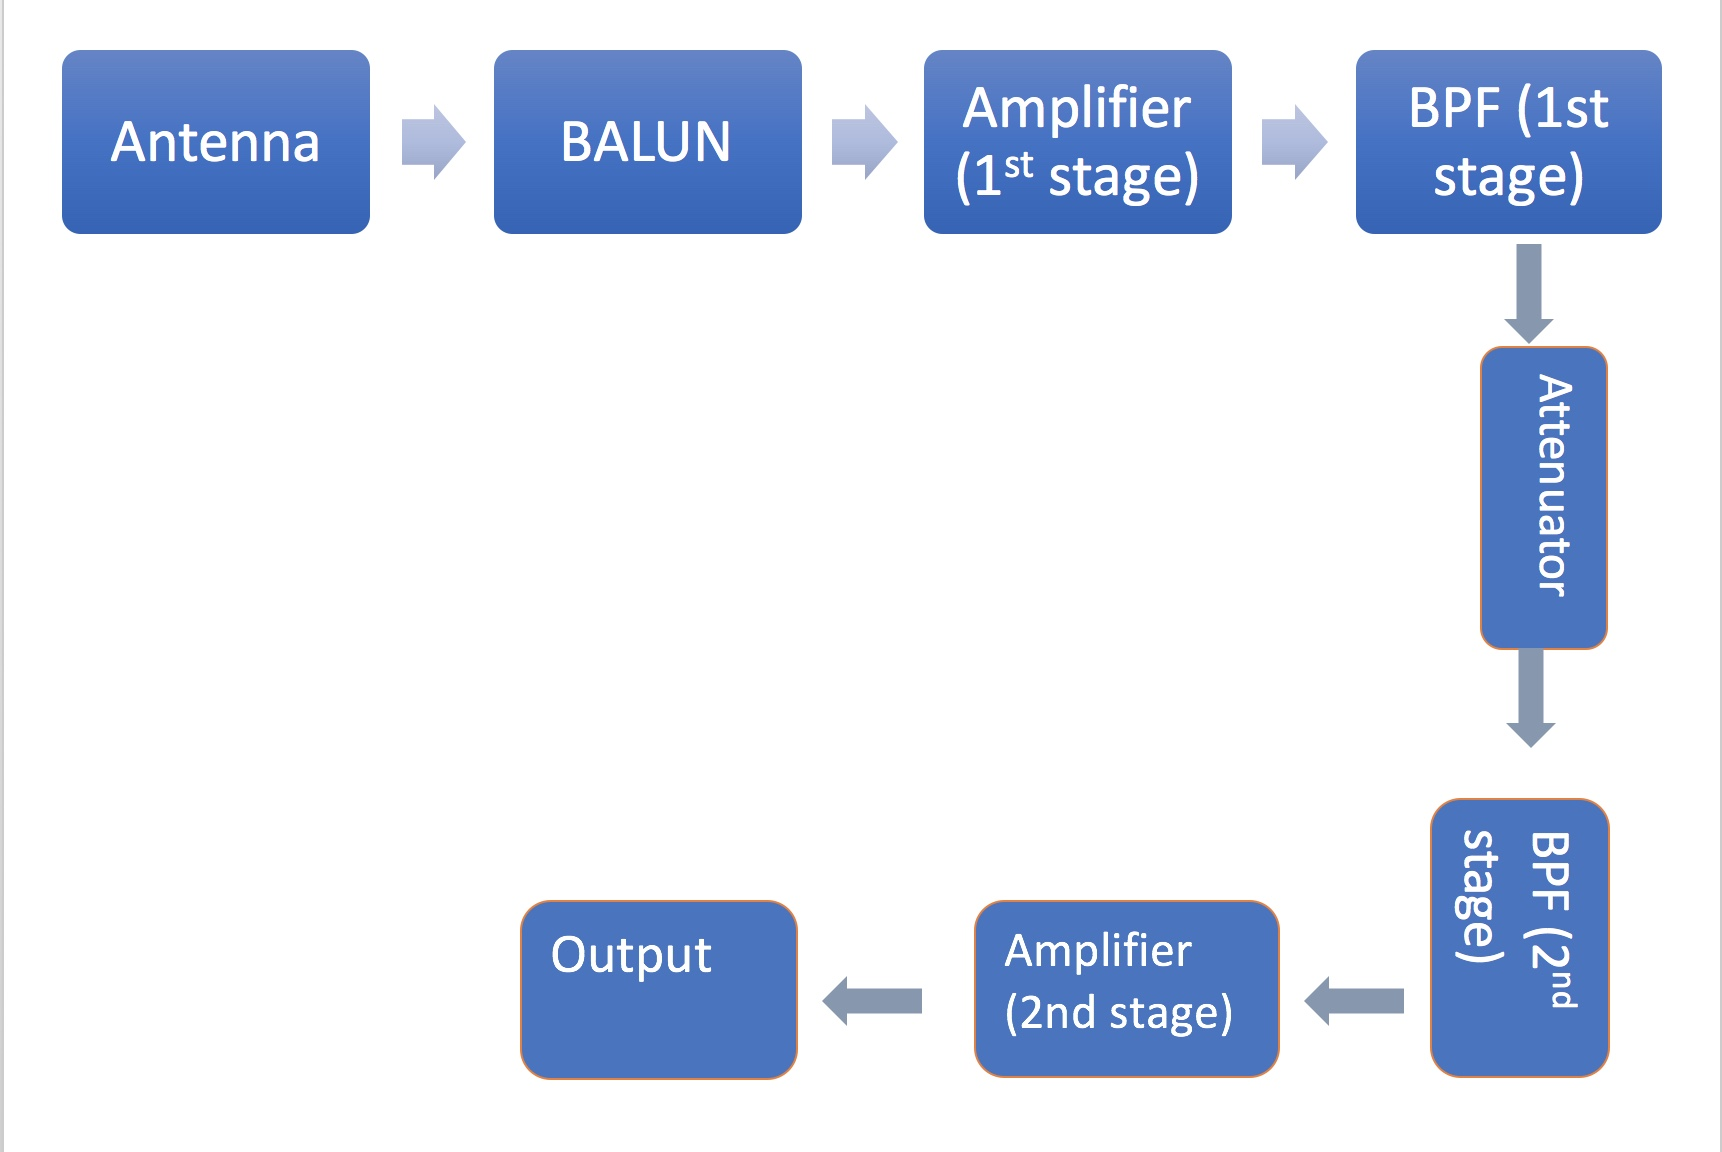
\includegraphics[width=5in,height=3.5in]{Sig_high_freq.jpeg}

		Fig.1 signal chain diagram
		\end{center}
	    
	    \item  We visualize the output thrugh FieldFox Spectrum analyzer (manufacturer: Keysight Technologies). We find out the lowest value of attenuator in order to avoid the 'ADC Saturation' warning. In addition to it, the analyzer sets an internal attenuation of 10dB. 
		
		\begin{center}
			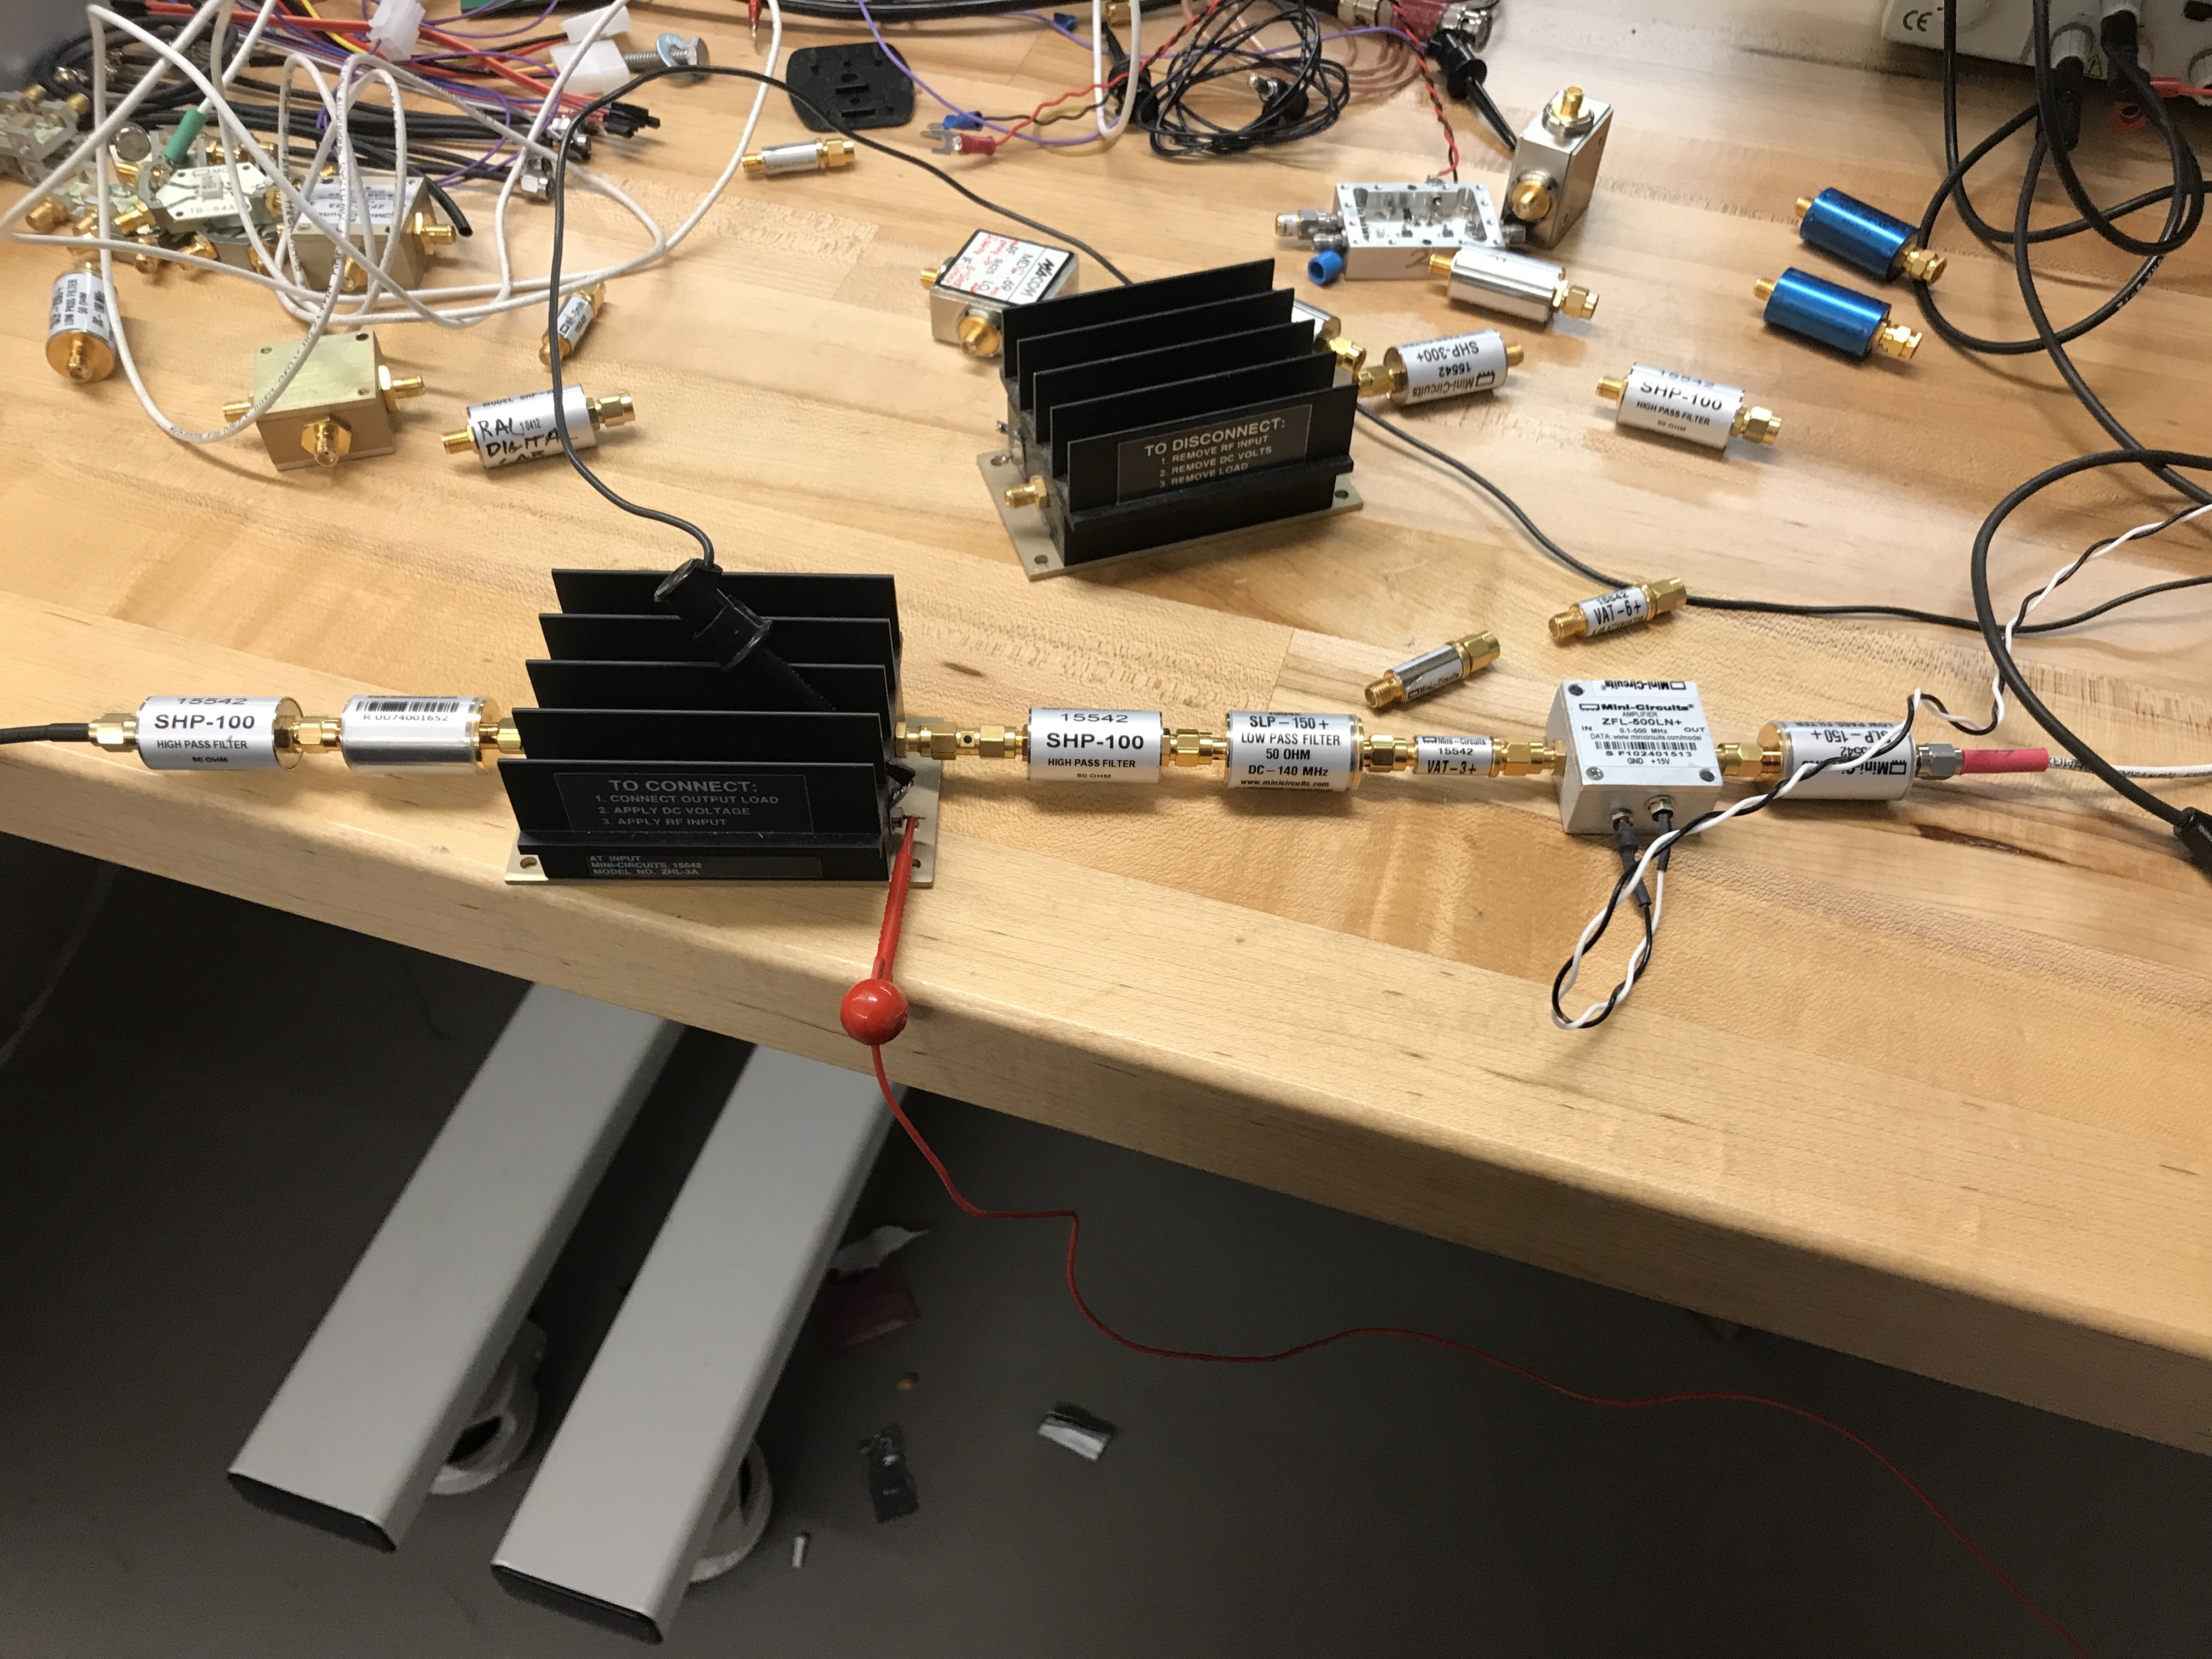
\includegraphics[width=5in,height=3.5in]{sig_chain.jpeg}
			
			Fig.2 Assembled signal chain 
		\end{center}
	
		\item We connected the antenna feed,followed by a passive Balun ( which does not require DC ) to the signal chain. This is the 'Absorber Off' state.
		
		\begin{center}
		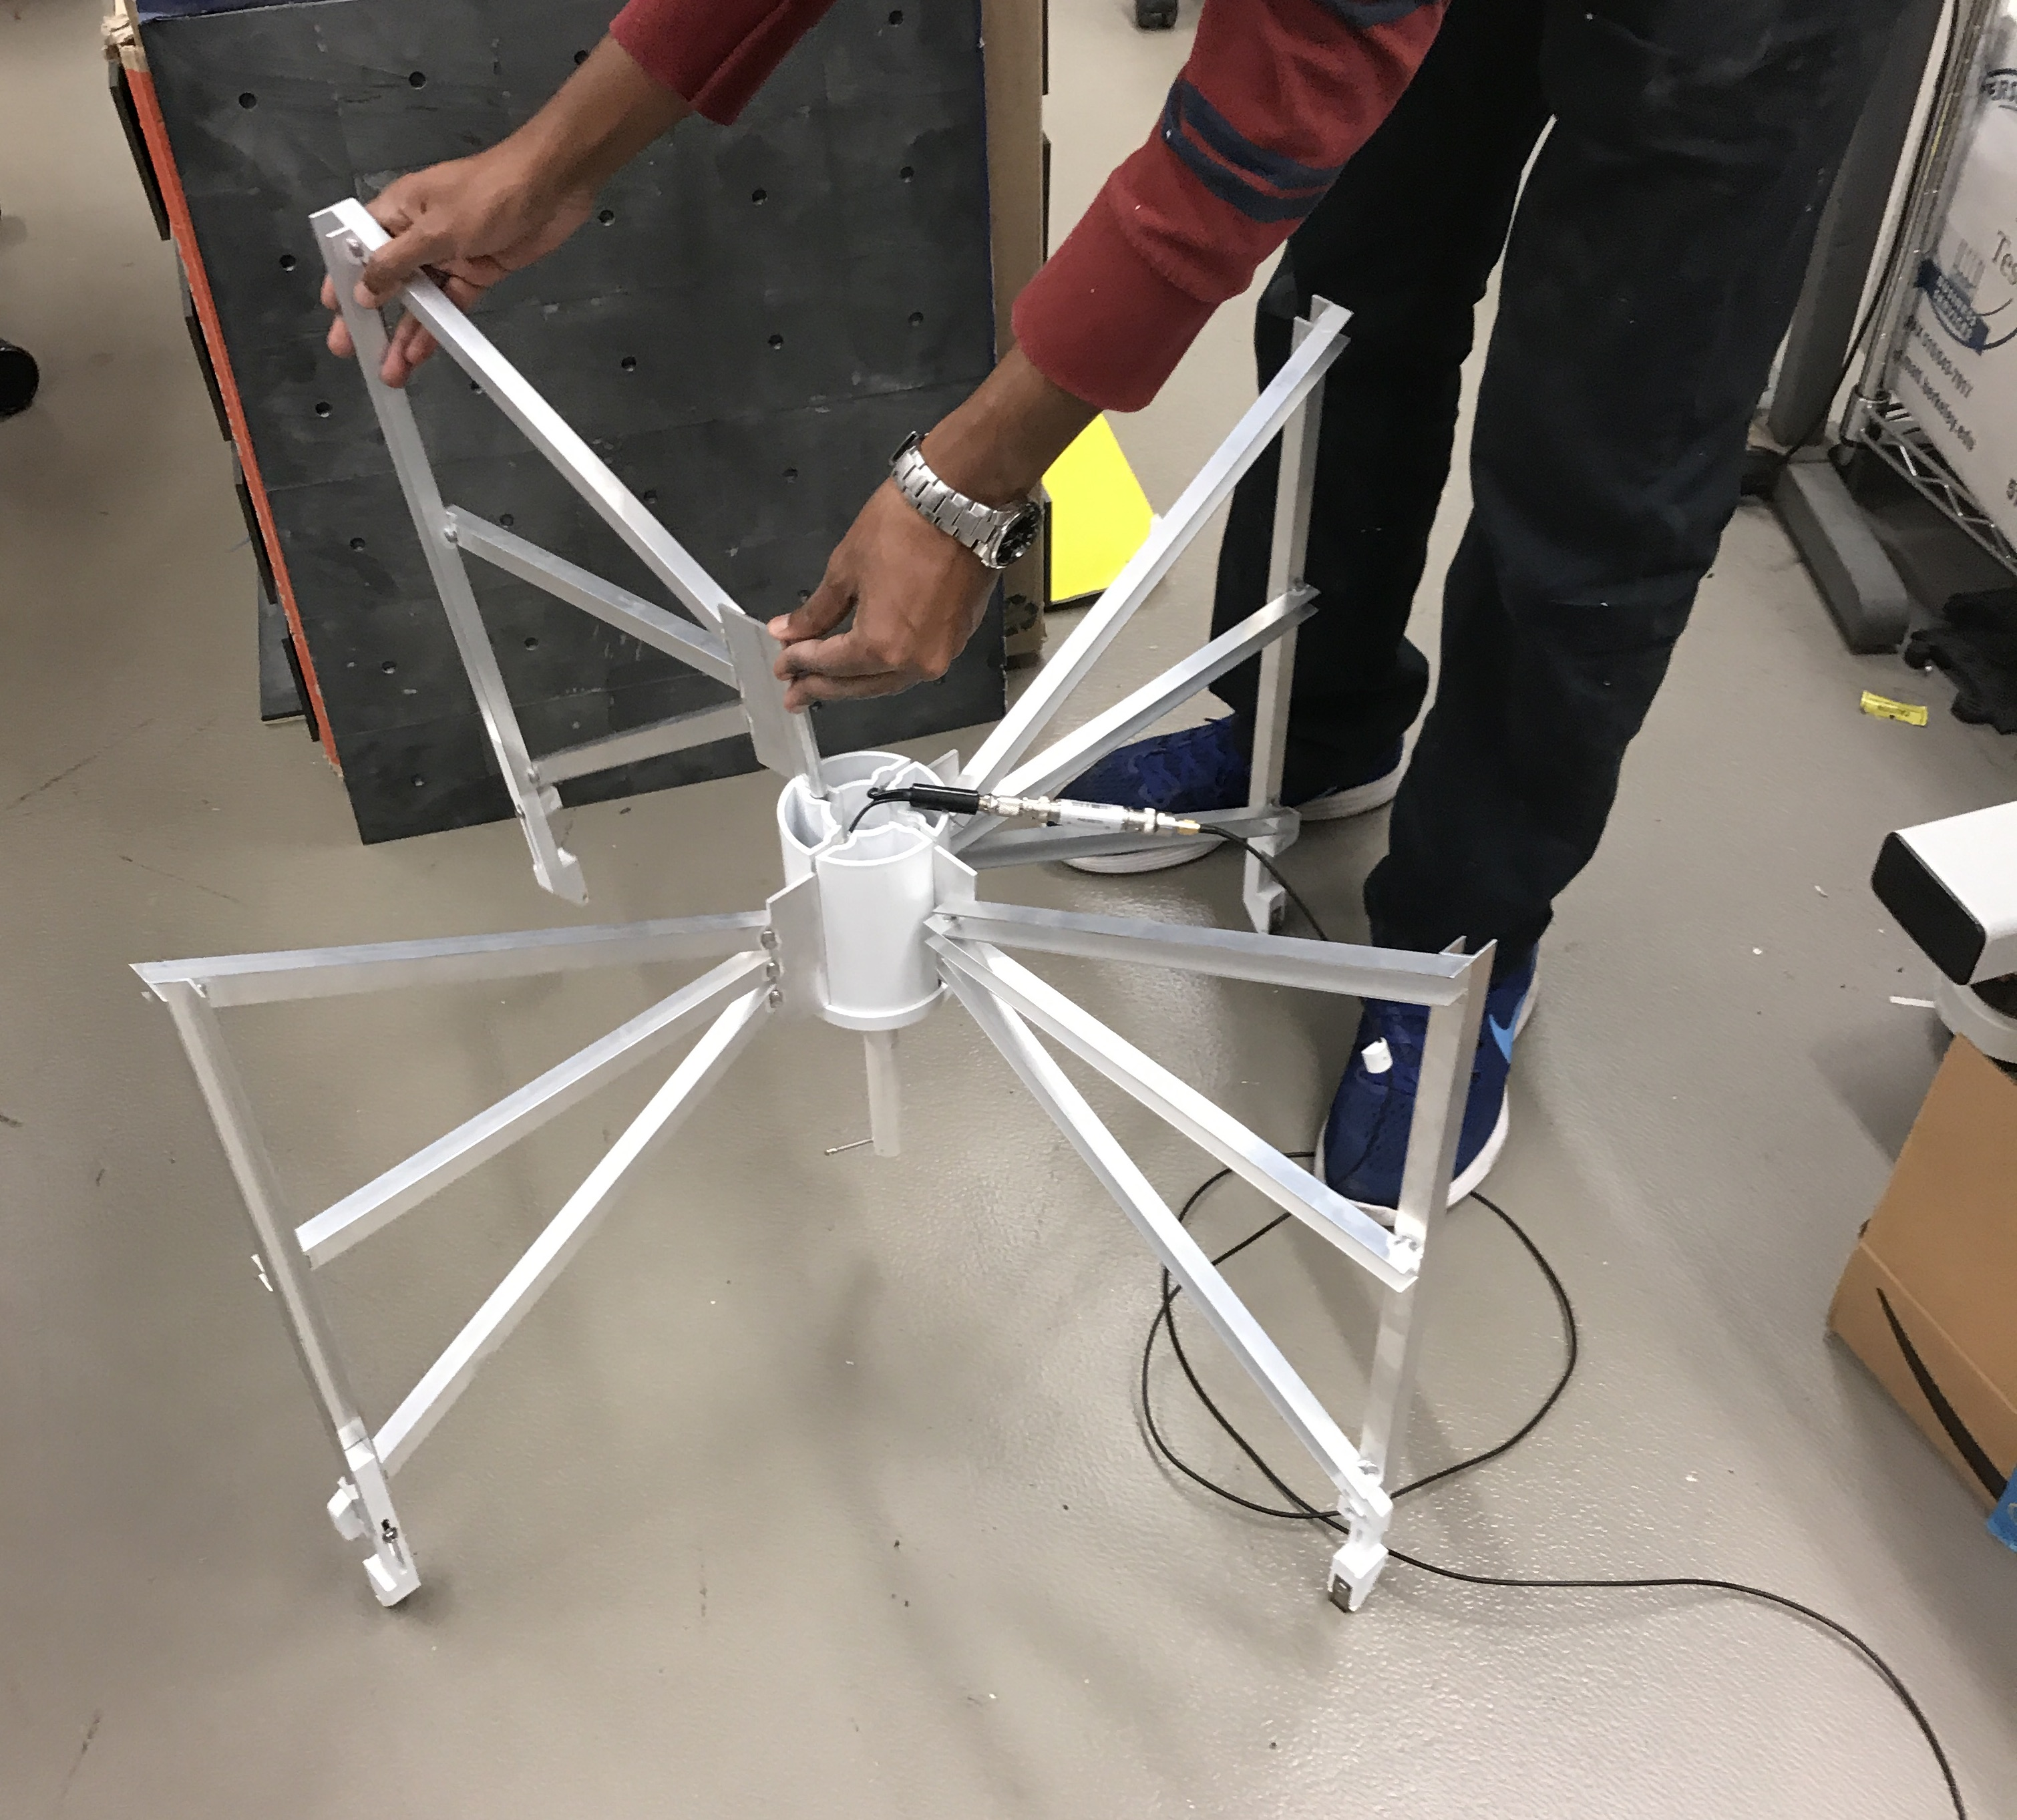
\includegraphics[angle=0,width=5in,height=3.5in]{feed.jpeg}
			
			Fig.3 Raj putting the feed elements together
		\end{center}	
		
	Under this configuration,the antenna is affected by the huge amount of RFI from the surroundings. The most  prominent ones are from the FM band. On the higer side,	some RFIs are so strong that we see them even after the filter cut-off.
		
		\item Then the antenna is put inside a cardboard box,with all its sides covered with absorber (Ferrite tiles). This gives us the 'Absorber On' measurement.
		\begin{center}
			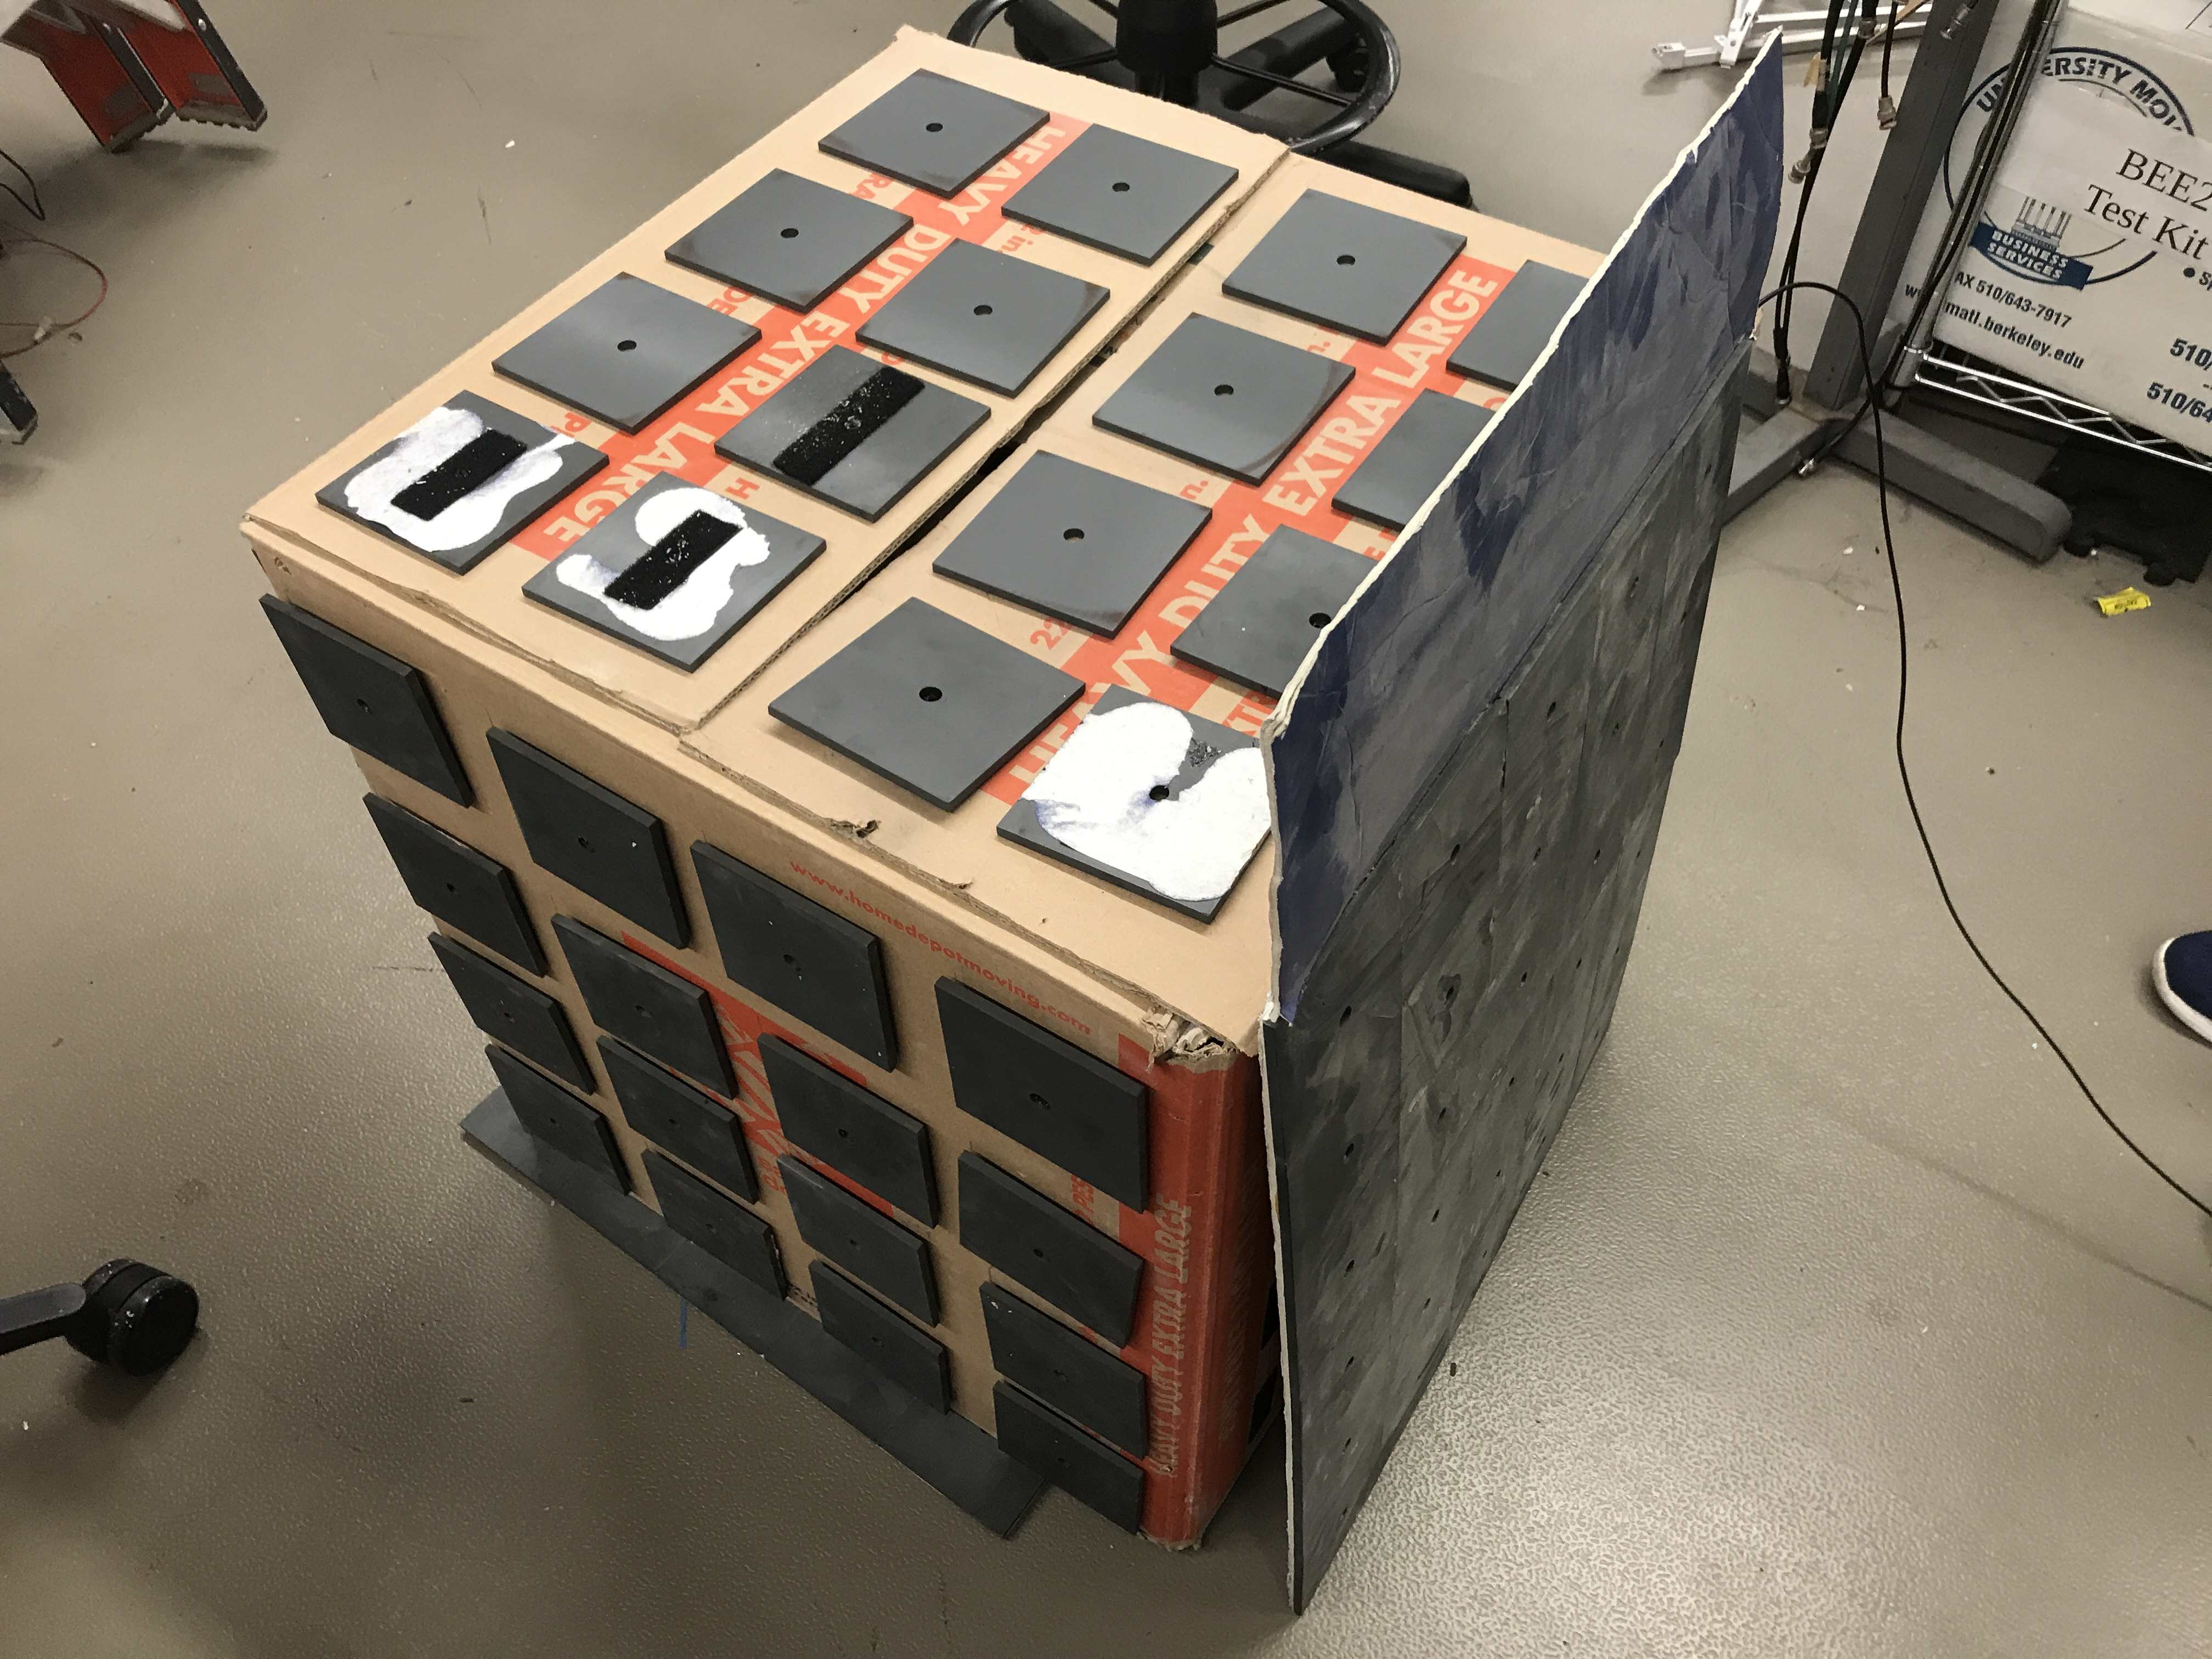
\includegraphics[width=5in,height=3.5in]{box.jpeg}
			
			Fig.4 Antenna covered by absorber tiles
		\end{center}
	
		
		\item When we compared the two results,we saw that the absorbers attenuated the RFI power level slightly.
	
	\begin{center}
		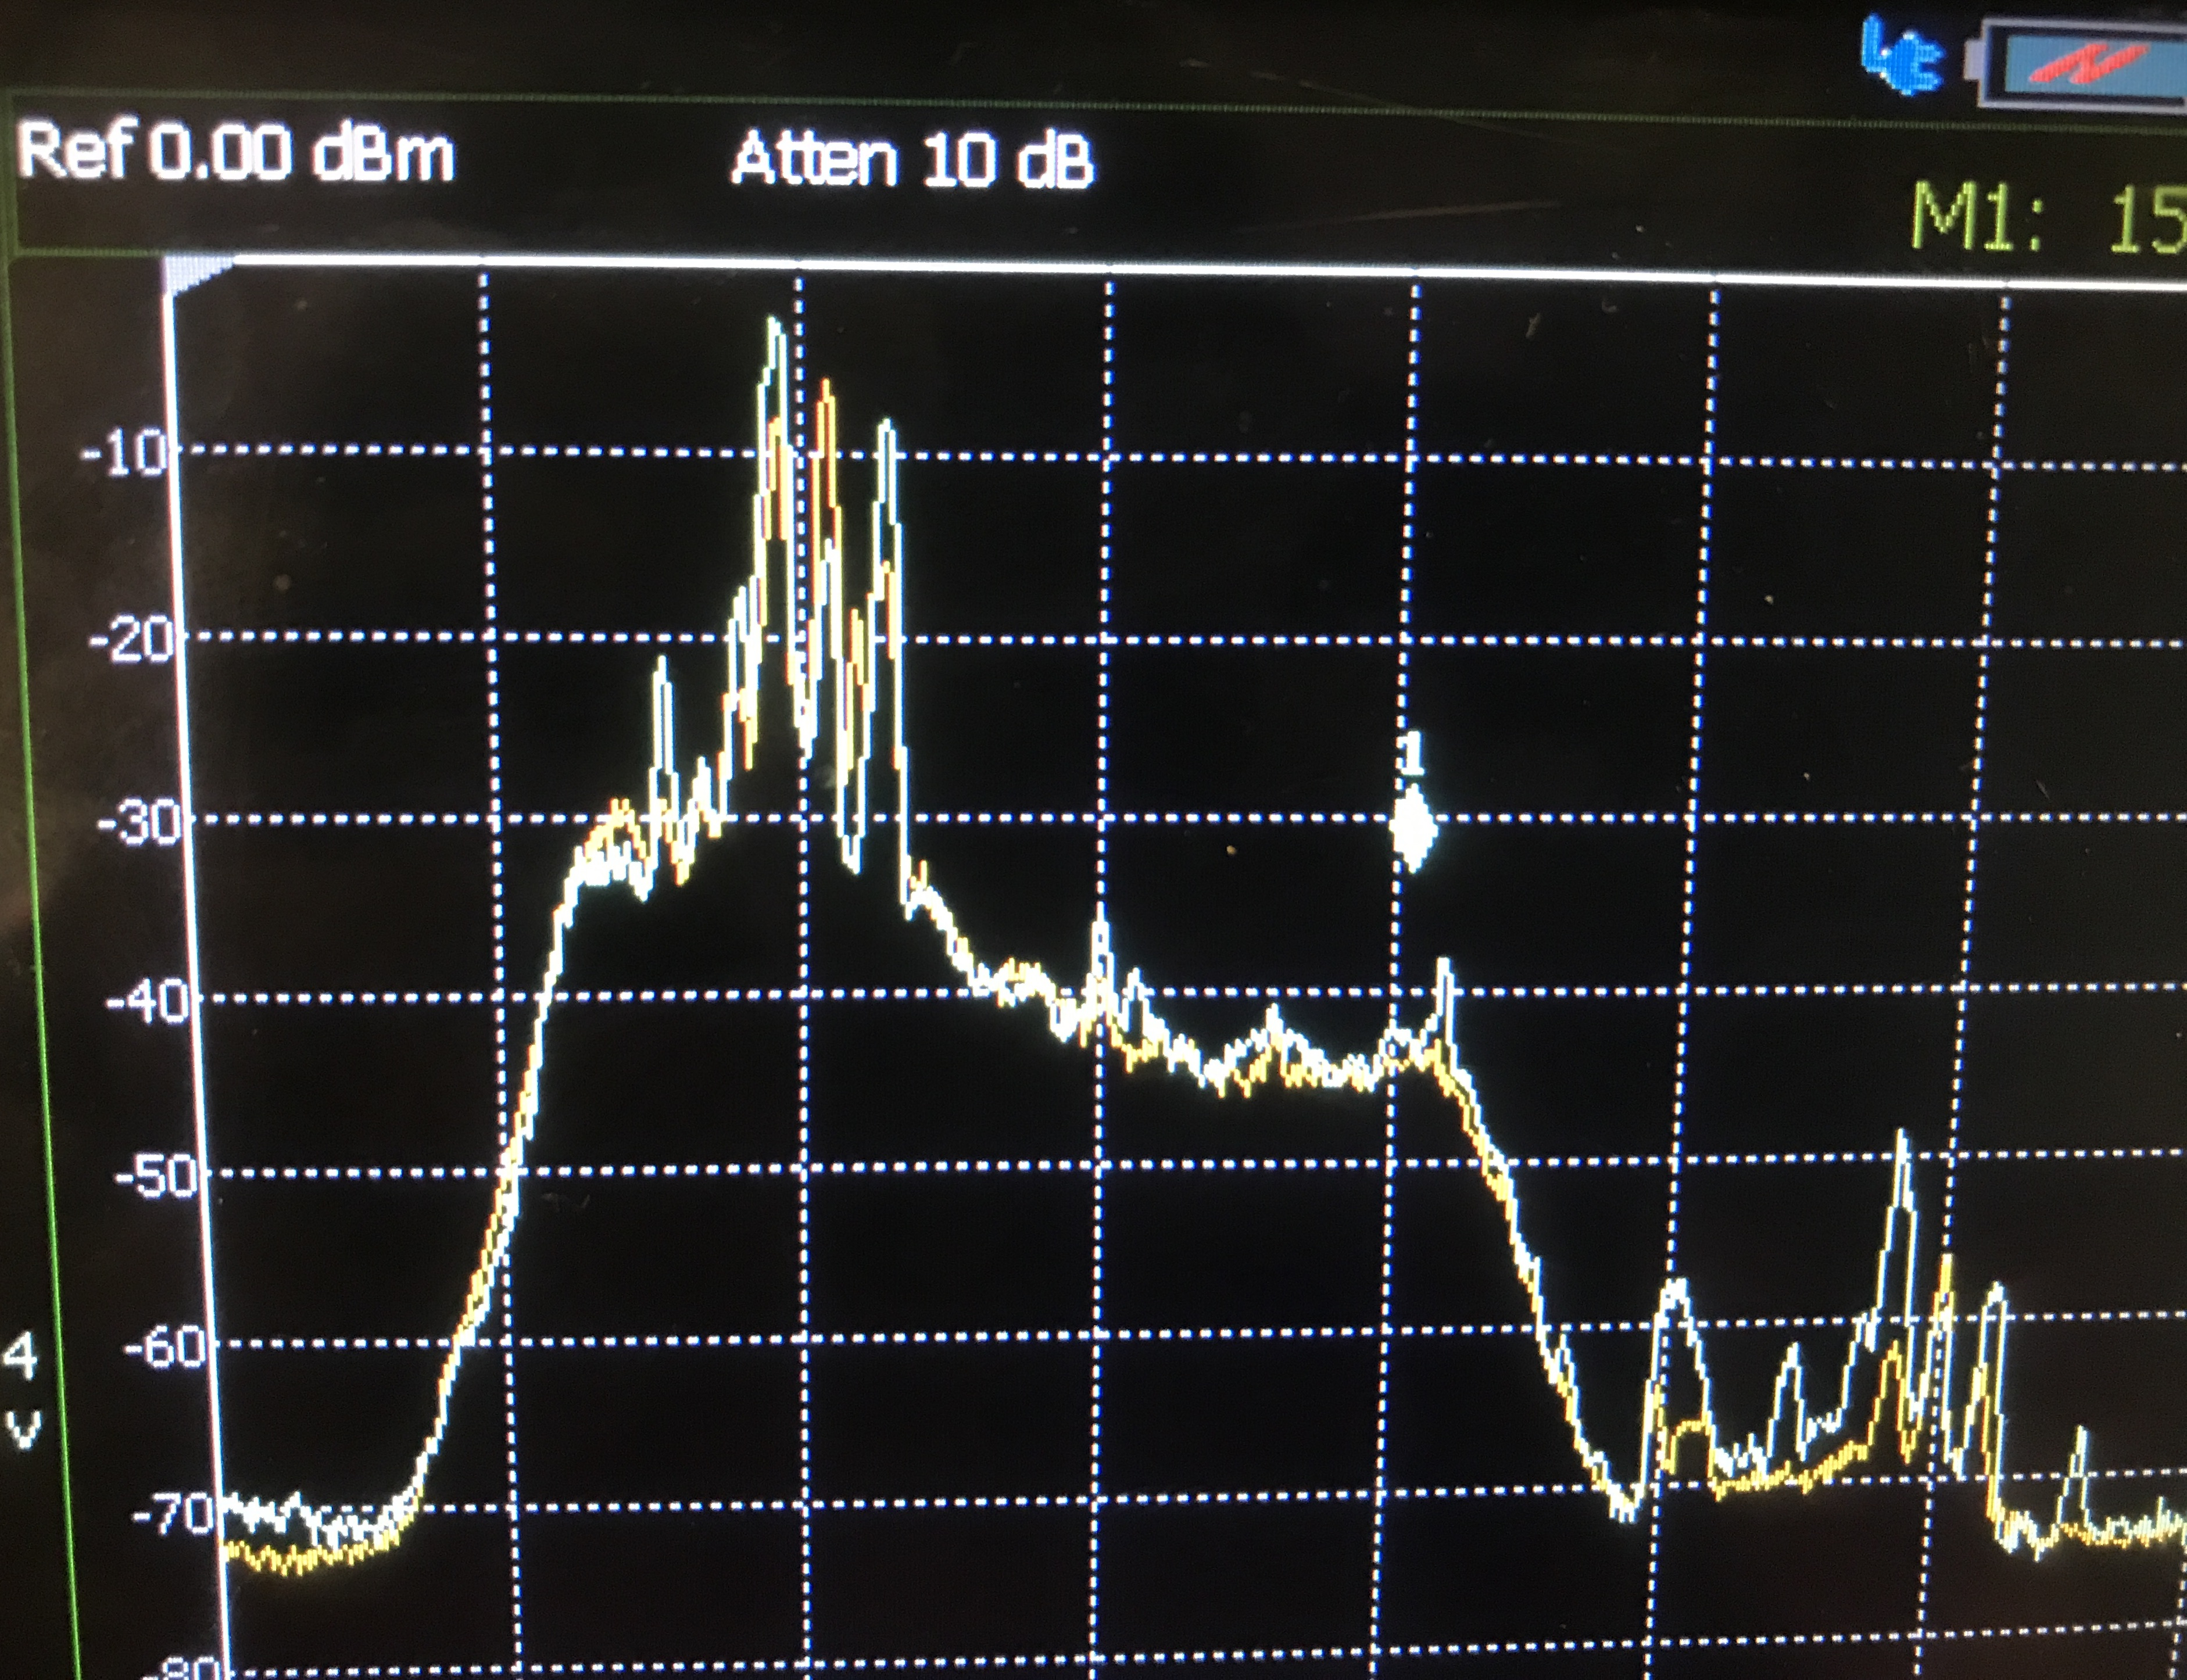
\includegraphics[width=5in,height=3.5in]{On_Off.JPG}
		
		Fig.5 'Absorber On' Vs. 'Absorber Off' measurements
	\end{center}
 	
 		\item We compared these results with that of a signal injected into the signal chain by a noise generator. We set the appropriate attenuation at the generator to get the similar power level. This would show us the clean band-pass.
 		
 		\begin{center}
 			\includegraphics[width=5in,height=3.5in]{combined.JPG}
 			
 			Fig.6 Antenna signal vs. Noise generator
 		\end{center}
 	\end{itemize}
 
 \section{Conclusion}
 We can conclude that the signal chain works as expected. Next,we need to do the interferometric measurement using this setup in lab,if possible. However,we need to keep in mind a few things:
 
 \begin{enumerate}
 	\item The 10 dB attenuation from analyzer will not be present when we use the SNAP board. 
 	\item SNAP ADC has a certain power level defined for the input signal. So,we have to pick the attenuator values accordingly.
 	\item Passive Baluns are easier to operate and contribute to a less complex signal chain. Hence, we should consider using passive Baluns in our experiments.
 	
 \end{enumerate}
 
 
\end{document}